
%% CLASS MANUAL FOUND IN http://blog.poormansmath.net/latex-class-for-lecture-notes/ %%
%% CLASS AUTHOR Stefano Maggiolo %%
\documentclass[english,course]{Notes}
\title{MATHEMATICS 1S}
\subject{Mathematics}
\author{Joao Almeida-Domingues}
\email{2334590D@student.gla.ac.uk}
\speaker{}
\date{10}{01}{2019}
\dateend{24}{05}{2019}
\place{University of Glasgow}
\usepackage[backend=biber, style=reading]{biblatex}
\bibliography{1Sbiblio}

\graphicspath{{assets/}}
	 
 %%%%% GENERAL MATHEMATICAL NOTATION SHORTCUTS %%%%%
 
\newcommand{\n}{\mathbb{N}}
\newcommand{\z}{\mathbb{Z}}
\newcommand{\q}{\mathbb{Q}}
\newcommand{\cx}{\mathbb{C}}
\newcommand{\real}{\mathbb{R}}
\newcommand{\field}{\mathbb{F}}
\newcommand{\ita}[1]{\textit{#1}}
\newcommand{\oneton}{\{1,2,3,...,n\}}
\newcommand\ef{\ita{f} }
\newcommand\inv[1]{#1^{-1}}
\newcommand\setb[1]{\{#1\}}
\newcommand\en{\ita{n }}
%\renewcommand\qedsymbol{QED} %QED instead of square

%%%%%%%%%%%%%%%%PACKAGES%%%%%%%%%%%%%%%%%%%%%%%%%%%%%
%\usepackage{lipsum}  

\usepackage{amsmath,amsthm,amssymb,graphicx,mathtools,tikz} %maths
\usepackage{hyperref,framed,color,fancybox} %layout


% framed :  \begin{shaded,frame,snugshade or leftbar} \definecolor{shadecolor}{rgb}{XYZ} to change color
%fancybox: \shadowbox,ovalbox or doublebox
%\extra for Extra content layout box
%%%%%%%%%%%%%%%%%%%%%%%%%%%

%%%CLASS SHORTCUTS%%%%
%\lecture{day}{month}{year} for margin note 
%\begin{theorem} sdfsdf\end{theorem}  --> \theorem
%\begin{proposition} dfsdfs\end{proposition} --> \prop
%\begin{lemma} dsfsd \end{lemma} --> \lem
%\begin{corollary} f ffew \end{corollary}
%\begin{definition} fwewef w \end{definition} --> \defn
%\begin{example} feww e\end{example} --> \ex
%\begin{exercise} wefwe \end{exercise}
%\begin{remark} wef we \end{remark} --> \rem
%\begin{fact} wefe \end{fact}
%\begin{problem} wef ew \end{problem}
%\begin{conjecture} ewfew \end{conjecture}
%\begin{claim} few w \end{claim}
%\begin{notation} fewf \end{notation} --> \nota
%\mymarginpar for scriptsize margin

\begin{document}
\newpage

\section{Taylor \& McLaurin Series}

\lecture{10}{01}{2019}

\subsection{Geometric Interpretation}
\textbf{Motivation:} Some functions cannot always be easily evaluated (e.g. $\cos(47)$), polynomial functions on the other hand are, one plugs the values in, and after performing some arithmetic  gets an output. Taylor series \ref{taylor:taylordef} are a \textbf{tool for approximating functions, by converting them into polynomials} .\footnote{https://media.giphy.com/media/zZYEX0w4bj8hG/giphy.gif} \\


\par{We cannot however choose any polynomial, it must be one which closely resembles the original function. Our first question should then be "When are two functions equal?". Obviously, two functions are equal if they have all points in common, or to put it another way, if they have the same shape. It follows then, that two functions will be \ita{approximately} equal if their shapes match \ita{approximately}.} \\

\par{ Let $f(x) = \cos(x)$ , be the function which we want to approximate near $x = 0$. Let $g(x) = c_0 + c_1x^1 + c_2x^2 + c_3x^2 + \dots $ be a general polynomial.} \\ As it stands we seem to have two different problems (1) We'll need to find the constant terms which make $g(x)$ have a similar shape to that of $f(x)$. (2) We must find a way to obtain a value of the sum, which is not possible for an infinite polynomial.

\begin{enumerate}
	\item Since we know how to evaluate $sin(0) = 0$ , we know that : 
	$$g(0) = 0 \iff g(0) = c_0 + c_1(0)^1 + c_2(0)^2 + c_3(0)^2 + \dots$$ 
	But since any higher order terms \ita(h.o.t) will all be $0$ , we find that $c_0 = 0$
	
	At this stage we have the following:


\begin{figure}[h]
\centering
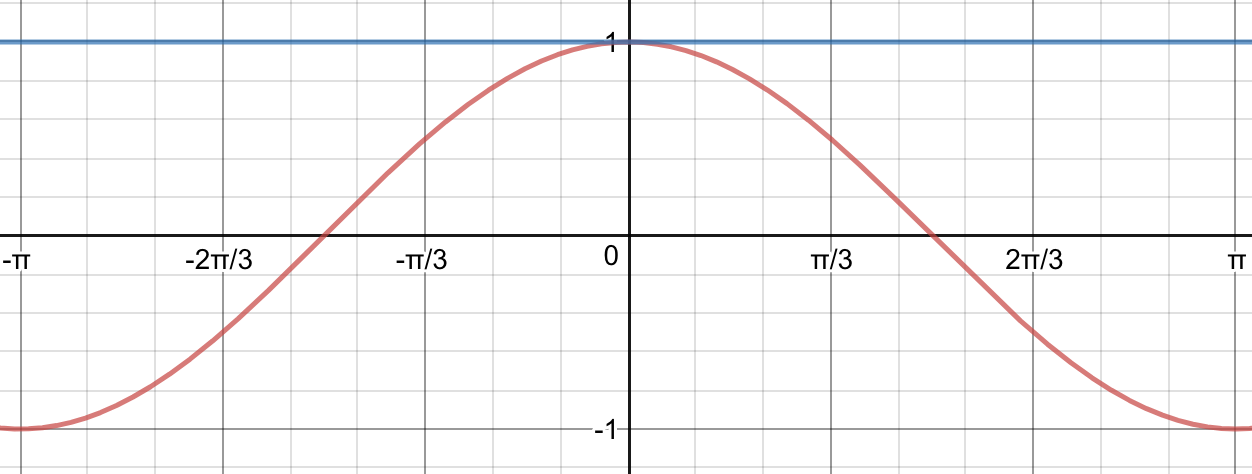
\includegraphics[width=0.5\textwidth]{taylor1st}
\end{figure}


\par{ This is far from a good approximation, but we have found one constant for our polynomial. Next we can think of other information we can get from $cos(x)$ near $x=0$. We know how to differentiate, hence he can get the rate of change of the function at $0$}

\item Finding the first order derivative for $f(x) \text{ and } g(x)$ we have that $f'(0) = -\sin(0) = 0$ and $g'(0) =  c_1 + 2c_2(0) + 3c_3(0)^2 + \dots = c_1$ . Again by equating the two derivatives we find that $c_1 = 0$. We now have: 

$$ g(x) = 1 + c_2x^2 + \cdots $$

\par{ Which did not help much, but we can still get more information, this time from the second-order derivative, and by repeating this process we'll get more and more terms for $g(x)$,and our approximation will be more and more accurate}

\item For up to the $6^{th}$ higher-order derivative we have that :

\begin{figure}[h]
\centering
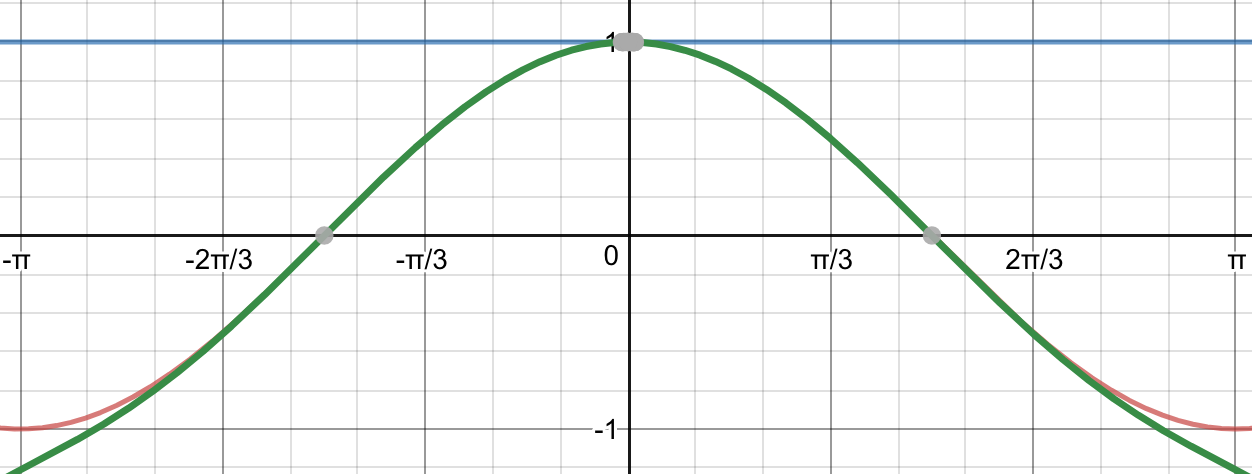
\includegraphics[width=0.5\textwidth]{taylor2nd}
\end{figure}


$$ g(x) = 1 + \frac{x^2}{2} + \frac{x^4}{24} + \frac{x^6}{720} $$

If we plugin a value into our polynomial, we find that the result is $\approx 98\%$ accurate comparing to the one obtained by a calculator. 

We still do not know "when to stop". For a periodic function like $\cos(x)$ this is sort of irrelevant, but for other functions which do not behave so regularly we can erroneously assume that our approximation is accurate anywhere in their domain, which in certain cases would be wrong \ref{taylor:rangeval}. How can we solve our \ita{infinite sum problem}

\item Lets first note that for each new term we generate, there seems to emerge a pattern. Every time we found a new higher order derivative , every other term we are not considering, remains unchanged *. \mymarginpar{*since they either differentiate to $0$ (l.o.t) or are multiplied by $0$ (h.o.t).} Furthermore, since $g(x)$ is a polynomial, every time we differentiate to find $c_n$ we find that the powers of \ita{h.o.t} accumulate, s.t. when we reach the $n^{th}$ term, the coefficient of $x$ is equal to n! which needs to be cancelled in order to obtain $c_n$, so the inverse is taken. So, at x = 0:

$$ c_n = \frac{1}{n!}f^{(n)}(0) \label{taylor:cN} $$

\nota{ $f'^{(n)}$: the $n^{th}$ order derivative}

\item \mymarginpar{*for example, the $18^{th}$ term of our example above yields 0.0000000002679245561}After coming to the conclusion above (\ref{taylor:cN}), we observe that if the series converges \ref{taylor:ratio} towards a limit, then as the \ita{h.o.t} become larger, they become less and less significant*. Let the first $n$ "significant" terms of the polynomial represent a \ita{truncated power series} \ref{taylor:powerSeries} \ref{taylor:taylorpoly} , and all higher order ones - $O(x^n)$ - or - $R_n(x)$ - be the \ita{remainder} of the series. Then if $ \lim_{n\to\infty}R_n(x) = 0$ , $f(x)$is just the sum of the series up until n.

\nota{$O(x^n)$ : All all the omitted terms are of $n^{th}$ order or higher in $x$}
\newpage
\subsection{Calculating}

\textbf{Putting it all together:}

\defn{Power Series\label{taylor:powerSeries} \ \ \ \ \ }{$ \sum _ { n = 0 } ^ { \infty } a _ { n } x ^ { n }$}

\defn{Taylor Series*\mymarginpar{*of $f$ at $a$}}{$$ \ \ \ \ \sum_{n=0}^{\infty}\frac{f^{(n)}(a)}{n!}(x-a)^n$$ \label{taylor:taylordef}}

\defn{Taylor Polynomial \label{taylor:taylorpoly}}{ A polynomial which higher order derivatives are designed to matchup with the original function (truncated Taylor series)}

\rem{Note that the example above evaluates the derivatives at $0$ because it is "cleaner" to do so, but we can start at any point where the value of the function is known. When starting at $0$ the series are called \textbf{McLaurin Series} \ref{taylor:mc} }

\defn{McLaurin Series \label{taylor:mc}}{$$ \ \ \ \ \sum_{n=0}^{\infty}\frac{f^{(n)}(0)}{n!}(x)^n$$}

\defn{Range of Validity\label{taylor:rangeval}}{ The values of $x$ for which the infinite sum exists and is equal to $f(x)$} \mymarginpar{TO DO: Method for finding it}
 
\end{enumerate}

 \extra{The Ratio Test \label{taylor:ratio} \begin{enumerate}
\item Convergent if $\lim_{n\to\infty} = \Big|\frac{a_{n+1}}{a_n}\Big| < 1$
\item Divergent if $ \lim_{n\to\infty} = \Big|\frac{a_{n+1}}{a_n}\Big| > 1$
\item Inconclusive if $ \lim_{n\to\infty} = \Big|\frac{a_{n+1}}{a_n}\Big| = 1$
\end{enumerate}}

\newpage
\lecture{11}{01}{2019}

\subsection{Important Series}

$$e ^ { x } = 1 + \frac { x } { 1 ! } + \frac { x ^ { 2 } } { 2 ! } + \frac { x ^ { 3 } } { 3 ! } + \frac { x ^ { 4 } } { 4 ! } + \cdots \quad x \in \mathbb { R }$$

$$\sin x = x - \frac { x ^ { 3 } } { 3 ! } + \frac { x ^ { 5 } } { 5 ! } - \frac { x ^ { 7 } } { 7 ! } + \cdots \quad x \in \mathbb { R }$$

$$\cos x = 1 - \frac { x ^ { 2 } } { 2 ! } + \frac { x ^ { 4 } } { 4 ! } - \frac { x ^ { 6 } } { 6 ! } + \cdots \quad x \in \mathbb { R }$$

$$\log ( 1 + x ) = x - \frac { x ^ { 2 } } { 2 } + \frac { x ^ { 3 } } { 3 } - \frac { x ^ { 4 } } { 4 } + \frac { x ^ { 5 } } { 5 } - \cdots \quad x \in ( - 1,1 ]$$

$$( 1 + x ) ^ { \lambda } = 1 + \left( \begin{array} { c } { \lambda } \\ { 1 } \end{array} \right) x + \left( \begin{array} { c } { \lambda } \\ { 2 } \end{array} \right) x ^ { 2 } + \left( \begin{array} { c } { \lambda } \\ { 3 } \end{array} \right) x ^ { 3 } + \cdots \quad x \in \left\{ \begin{array} { c c } { ( - 1,1 ) } & { \text { if } \lambda < 0 } \\ { \mathbb { R } } & { \text { if } \lambda \geqslant 0 } \end{array} \right.$$


\ex{Find the MacLaurin Series for $f(x) = e^x$}

\par{We start by noting that $f^{(n)}(x) = e^x$ . Hence evaluating it at $ x = 0 $, we get $f^{(n)}(o) = e^0 = 1$. Therefore we can find the constant terms of the series by applying \ref{taylor:cN}, giving us:}

$$ c_n = \frac{1}{n!}$$

and so,

$$ e^x = \sum^{\infty}_{n=0}\frac{x^n}{n!} = 1 + \frac{x}{1!} + \frac{x^2}{2!} + \frac{x^3}{3!} + \dots$$

\ex{Find the Maclaurin Series for $g(x) = \log(1+x)$}

\begin{enumerate}
	\item We'll start by substituting $(1+x)$ so that we can observe the behaviour of the more general logarithm.
	
	Let $1 + x = y$ , then we have the common $\log$ derivative, $g(y)'=(\log(y))' = \tfrac{1}{y}$. What of the $n^{th}$ derivative? By differentiating the next 3 terms we notice a pattern emerging:
	
	\begin{align*}
		&g''(y) = -y^{-2} \\
		&g'''(y) = 2y^{-3} \\
		&g^{iv}(y) = 2(-3)y^{-4}
	\end{align*}
	
Therefore we have:

$$ g^{(n)}(y) = (-1)^{n-1}(n-1)!y^{-n} $$

	\item Hence, by application of the chain rule we get:
	
	$$ g^{(n)}(x) = \frac{d^{(n)}}{dy} log(y) \times \frac{d}{dx} (1 + x) =  \frac{(-1)^{n-1}(n-1)!y^{-n}}{1} = \frac{(-1)^{n-1}(n-1)!}{(1+x)^n}$$
	
	\item Evaluating it at $x = 0$, gives us the following first 4 terms: $ 0 , 1 , -\frac{1}{2} , \frac{1}{3}$
\end{enumerate}

\par{So that we have the approximation being given by the series: $$x - \frac{x^2}{2} + \frac{x^3}{3}  + \dots$$}

\lecture{17}{01}{2019}
\subsection{Manipulation of Series}

\begin{enumerate}

	\item \textbf{Addition}
		$$f(x) + g(x) = \sum_{n=0}^{\infty}(f_n+ g_n) x^n$$
	
	\item \textbf{Multiplication}
		$$\begin{aligned} f ( x ) g ( x ) & = \left( \sum _ { n = 0 } ^ { \infty } f _ { n } x ^ { n } \right) \left( \sum _ { m = 0 } ^ { \infty } g _ { m } x ^ { m } \right) \\ & = \sum _ { n = 0 } ^ { \infty } \left( \sum _ { r = 0 } ^ { n } f _ { r } g _ { n - r } \right) x ^ { n } \end{aligned}$$
		
		\ex{$f(x) = \frac { e ^ { 2 x } } { 1 - x }$ first 3 terms of the McLaurin series}
		
		\par{First we note that the function can be seen as the multiplication of two separate functions $g(x) = e^{2x}$ and $h(x) = (1-x)^{-1}$. Since we know the series for $e^y$, let y = 2x so that we have:}
		\begin{align*}
		e^ y &= 1 + \frac { y } { 1 ! } + \frac { y ^ { 2 } } { 2 ! } + \frac { y ^ { 3 } } { 3 ! } + \frac { y ^ { 4 } } { 4 ! } + \cdots , \quad y \in \mathbb { R } \\
	& = 1 + 2 x + 2 x ^ { 2 } + \frac { 4 x ^ { 3 } } { 3 } + \frac { 2 x ^ { 4 } } { 3 } + \cdots , \quad x \in \mathbb { R }
	\end{align*}
			
	\begin{align*}(1-x)^{(-1)} = 1 + x + x^2 + x^3 + x^4 + \cdots\end{align*}
	
	\par{Hence,}
	
	$$(e^2x) (1-x)^{(-1)} = (1 + 2 x + 2 x ^ { 2 } + \frac { 4 x ^ { 3 } } { 3 } + \frac { 2 x ^ { 4 } } { 3 } + \cdots) (1 + x + x^2 + x^3 + x^4 + \cdots) $$
	
	\par{Now we inspect which terms, when multiplied, will result in degree 3 or less and ignore the \ita{h.o.t}. So that we have:}
	
	$$ (e^2x) (1-x)^{(-1)} = 1 + 3 x + 5 x ^ { 2 } + \frac { 19 } { 3 } x ^ { 3 } + O(x^4) $$
	
	\item \textbf{Functions' Composition}
	
	$$f ( g ( x ) ) = \sum _ { n = 0 } ^ { \infty } f _ { n } \left( \sum _ { m = 0 } ^ { \infty } g _ { m } x ^ { m } \right) ^ { n }$$
	
	\ex{$\log ( \cos x ) \text { up to the term } x ^ { 6 }$}
	
	\par{Again, the underlining idea is to try and rewrite the expression so that we can use one of the simpler, known series.}
	
	$$ \log ( \cos x ) = \log \left( 1 + \boxed{( - 1 + \cos x )} \right) = \log ( 1 + y ) $$
	
	\par{Now it's possible to use the series for $ \log(1+x)$ that we've seen above.}
	
	$$ \log ( 1 + y ) = y - \frac{y^2}{2} + \frac{y^3}{3} + O(x^4) $$
	
	\par{ Note however, that $y$ must still satisfy the range of validity for the $\log$ function. Hence,}
	
	$$- 1 \leqslant - 1 + \cos x \leqslant 1 \iff 0 \leqslant \cos x \leqslant 2 $$
	
	\par{Finding the series for the inner function $1-\cos(x)$, gives us:}
	
	$$\begin{aligned} - 1 + \cos x & = \cancel{- 1} +  \left( \cancel{1} - \frac { x ^ { 2 } } { 2 ! } + \frac { x ^ { 4 } } { 4 ! } - \frac { x ^ { 6 } } { 6 ! } + O(x^7) \right) \\ & = - \frac { x ^ { 2 } } { 2 ! } + \frac { x ^ { 4 } } { 4 ! } - \frac { x ^ { 6 } } { 6 ! } - O(x^7) \end{aligned}$$
	
	\par{Finally, let $g(x) = 1- \cos(x)$ and $f(x) = \log(1+y)$ substituting $g(x)$ back into the series of $f(x)$ by application of the formula for composite series. We have,}
	
	$$\begin{aligned}
		\log\left(\cos(x)\right) &= y - \frac { 1 } { 2 } y ^ { 2 } + \frac { 1 } { 3 } y ^ { 3 } - \frac { 1 } { 4 } y ^ { 4 } + \cdots \\
			&= \left( - \frac { x ^ { 2 } } { 2 ! } + \frac { x ^ { 4 } } { 4 ! } - \frac { x ^ { 6 } } { 6 ! } - \cdots \right) - \frac { 1 } { 2 } \left( - - \frac { x ^ { 2 } } { 2 ! } + \frac { x ^ { 4 } } { 4 ! } - \frac { x ^ { 6 } } { 6 !} + \cdots \right) ^ { 2 } +  \\ & \ \frac { 1 } { 3 } \left( - \frac { x ^ { 2 } } { 2 ! } + \frac { x ^ { 4 } } { 4 ! } - \frac { x ^ { 6 } } { 6 !} + \cdots \right) ^ { 3 } + \cdots \\
			&= - \frac { x ^ { 2 } } { 2 } - \frac { x ^ { 4 } } { 12 } - \frac { x ^ { 6 } } { 45 } + O(x^7)
			\end{aligned}$$

\end{enumerate}

\lecture{18}{01}{2019}

\mymarginpar{TODO: Error using remainder, limits, complex arguments}

\section{Integration}

\lecture{24}{01}{2019}

\subsection{The Area Under The Curve}

\par{The \textbf{key idea} of this section is to understand that we can \ita{approximate} the area of non-regular shapes, like curves, by inscribing (or out-scribing) a regular polygon of which we can easily calculate the area of}

\rem{It is self-evident that the more polygons we use, the closer we get to completely cover the area under the curve.~\label{area:accurate}}

\rem{Following from (\ref{area:accurate}) , it is also clear that by using the notion of limit  (just like we saw in the chapter before) we should expect the total area to tend towards a number, i.e. by using a very large number of polygons (as $n \to \infty$) the overall area covered is equal to that of the curve}

\ex{Estimating the area under the curve $f(x) = x^2$ between 0 and 1}

\par{Let's start by comparing the estimates when using 4 and 16 rectangles with their left edges touching the curve.}

\begin{enumerate}
	\item{Calculating the width of the rectangles: We need to split the interval given $[0,1]$ into 4 and 16 equal parts. Let $\delta x$ represent the width for the 4-way split, and $delta y$ the 16-way split.}
	
	$$\delta x = \frac{1-0}{4} = \frac{1}{4} \quad \quad \delta y = \frac{1-0}{16} = \frac{1}{16}$$
	
	\item{Calculating the heights for each rectangle: Note that to calculate the height, all we need to do is to evaluate $f(x)$ where the rectangle and it meet. Since we've decided to draw the first rectangle starting its left-edge from $0$ and given that they'll have fixed width, we find that the height for a general $n^{th}$ rectangle is given by $0 + (n-1) (\frac{1}{4})$. Such that:
	
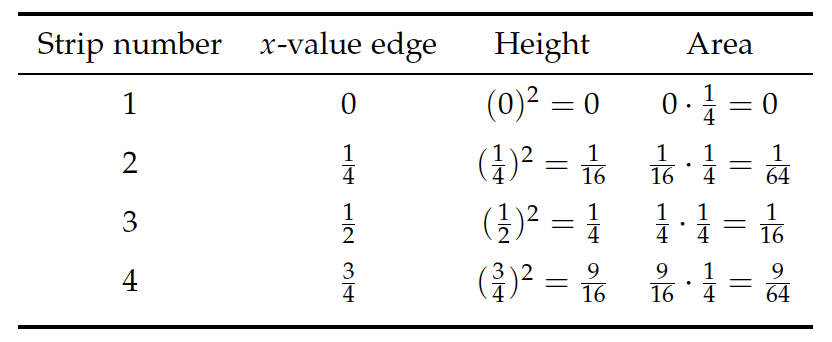
\includegraphics[width=15em]{area4strips}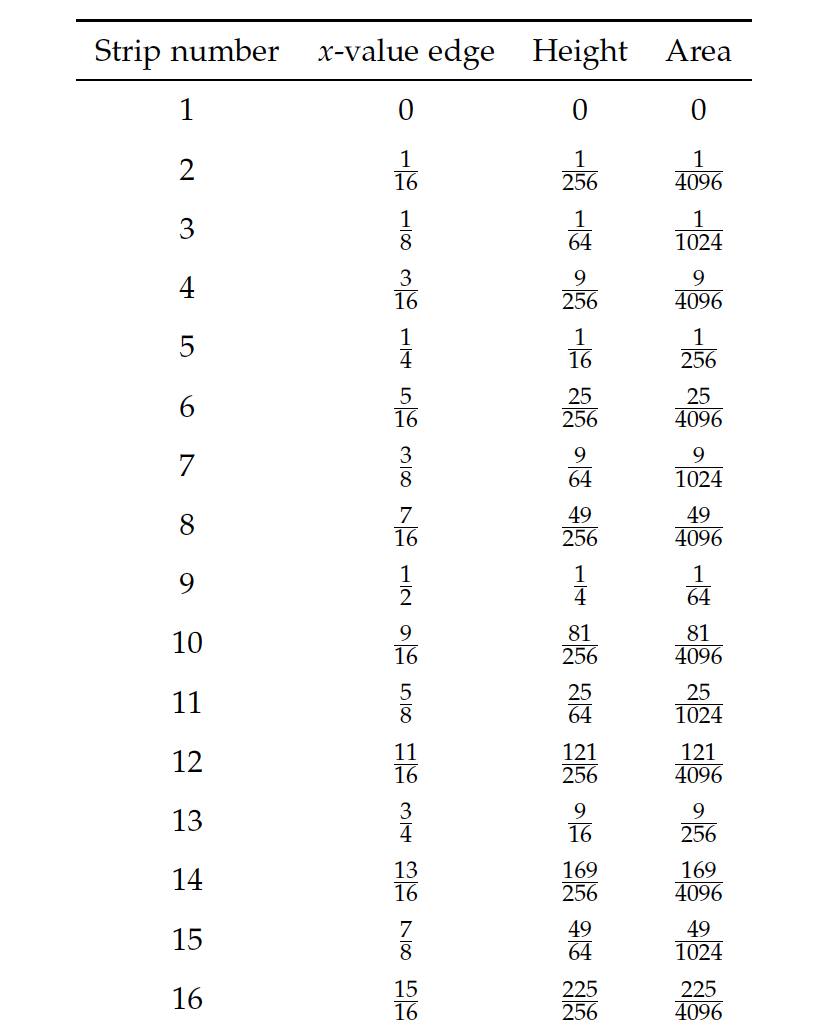
\includegraphics[width=15em]{area16strips}
}

	\item{Summing the areas $(R_n)$ of the rectangles to get an approximation of the area under the curve, we get:
	
	$$R_4 = 0.21875 \quad \quad R_16 = 0.302734375 $$
	
	
	}
	

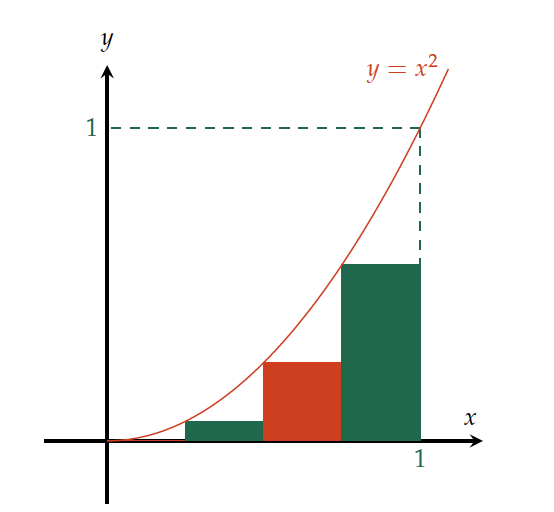
\includegraphics[width=15em]{area4strips2} 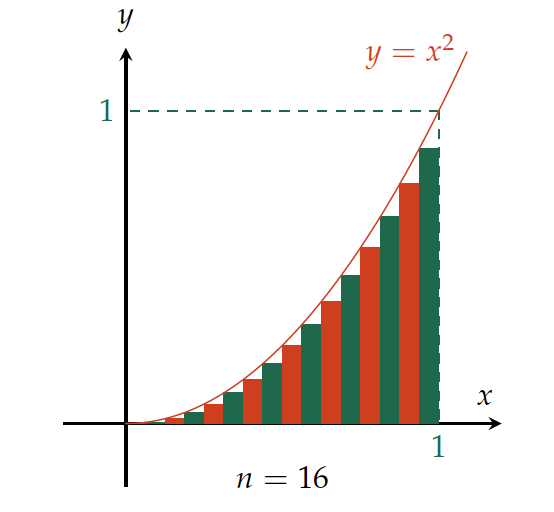
\includegraphics[width=15em]{area16strips2}
	
\end{enumerate}

\par{Note as remarked above, that by increasing the number of rectangles the area under the curve not accounted for decreases, therefore the approximation becomes more accurate. In fact, we can see that by very large numbers the area will tend towards $\tfrac{1}{3}$, giving us the precise area}

\rem{We chose to draw the rectangles matching their left edges with points in the curve, but we could equally have chosen the right edge or the middle point. The difference between the accuracy of the left and right edge approach depends of the shape of the curve. Choosing the middle point will however, always give us the best estimate, since it overestimates from one side, but it "compensates" by underestimating on the other.}
\newpage
\subsection{Calculating the Area by Evaluating the Limit of $R_n$}

\par{We can use our knowledge of series from 1R and from the previous chapter to evaluate the sum of a very large number of polygons, to get an exact value of the area under the curve}

\ex{Show that $\lim_{n \to \infty} R_n = \frac{1}{3}$

\par{By using a k number of strips, we have that their width is given by $\frac{1}{k}$, and the left edge value of the $j^{th}$ strip is then given by $0+(\frac{j}{k})^2$ or simply $(\frac{j}{k})^2$ since we are starting at $ x = 0 $. Finally the area of each strip is given by $\frac{1}{k} \cdot (\frac{j}{k})^2$ and their sum $(R_k)$:}

$$R_k = 0 + \frac{1}{k^2} + \left(\frac{2}{k}\right)^2 + \dots + \left(\frac{k-1}{k}\right)^2 = \frac{1}{k^3} \sum_{j=1}^{k-1}j^2$$

\rem{Remember the \textbf{sum of squares} \scriptsize{see algebra \ita{5.6}} \normalsize: $$\sum_{l=1}^{n} l^2 = \frac{n(n+1)(2n+1)}{6}$$}
}

\par{Hence:}

\begin{align*}
 R_k &= \frac{1}{k^3} \sum_{j=1}^{k-1} (k-1)^2 \\ 
 &= \frac{(k-1)((k-1)+1)(2(k-1)+1)}{6} \\
 &= \frac{2k^3 - k^2 - 2k^2 + k}{6k^3} \\
 &= \frac{1}{3} - \frac{1}{2k} + \frac{1}{6k^2}
 \end{align*}
 
 \par{So, as $n \to \infty$:}
 
 $$R_k = \frac{1}{3} - \underbrace{\frac{1}{\infty}}_0 + \underbrace{\frac{1}{\infty}}_0 = \frac{1}{3}$$
 
 \par{In general then, we have:}
 
 \defn{Area under the curve ~\label{area:limit}}{Let $y = f (x)$ be a continuous function and $a, b$ two values in the domain of $f$ . Then the area under the curve $y = f (x)$
between $x = a $and $x = b$ is the limit of the sum of the areas of the
rectangular strips:
 
 $$\lim_{n \to \infty}\sum_{j=0}^{n-1}f(x_j)\delta x$$}
 
 \newpage
 
 \subsection{Definite Integral}
 
 \defn{Definite Integral}{The limit of the sum of the areas of the rectangular strips (\ref{area:limit}) as the number of strips tend to infinity. $A$ is the integral from $ x = a $ to $x = b$ of $f(x)$ with respect to $x$ 
 $$ A = \int_{a}^{b} f(x) dx$$}
 
 \defn{Limits of Integration}{The interval $[a,b]$}
 
 \subsubsection{Riemann Sum Estimates}
 
 \par{Putting the 2 previous concepts together, we have the concept of \ita{Riemann Sums}}
 
 \defn{Riemann Sum}{An approximation to the area under the graph given by the sum of the areas of $n$ rectangles. Let $\delta x = \frac{b-a}{n}$ represent the width of each rectangle and $x_j = a + j\delta x$ represent the points where they meet the curve. Then, the area is given by:
 
 $$ \lim_{\delta x \to 0} \left(\sum_{j=0}^{j=n-1}f(x_j)\delta x\right) = \lim_{n \to \infty} \left(\sum_{j=0}^{j=n-1}f(x_j)\delta x\right) ~\label{definite:sum}$$}
 
\ex{
\par{Given $f(x) = x^3 - x$ , find its Riemann sum between $[0,2]$  with 6 intervals and its definite integral}

\begin{itemize}
	\item {We start by calculating $\delta x$, and the edges of each rectangle:
	
	$$\delta x = \frac{2-0}{6} = \frac{1}{3} \quad$$
	\begin{alignat*}{2}
		f(x_0) &= f(0) &= 0 \\
		f(x_1) &= f(\sfrac{1}{3}) &= -\sfrac{8}{27} \\
		f(x_2) &= f(\sfrac{2}{3}) &=  -\sfrac{10}{27} \\
		f(x_3) &= f(1) &= 0 \\
		f(x_4) &= f(\sfrac{4}{3}) &=  \sfrac{28}{27} \\
		f(x_5) &= f(\sfrac{5}{3}) &=  \sfrac{80}{27}
	\end{alignat*}}

	\item {The total estimated area is given by the sum of the strips' areas, hence:
	
	$$f(x) \approx \frac{1}{3} \left( - \frac{8}{27} - \frac{10}{27} +  \frac{28}{27} + \frac{80}{27} \right) \approx \frac{10}{9}$$
	}
	\newpage
	\item {To find the definite integral, we use the definition above (\ref{definite:sum})
	
	$$ \int_0^2 f(x) dx = \lim_{n \to \infty} R_n$$}
	
	\item{ Finding $R_n$:
	
		\begin{align*}
			R_n &= \sum_{j=0}^{n-1} f(x_j) \delta x \\
				&= \delta x \sum_{j=0}^{n-1} f(x_j) \\
				&= \frac{2}{n} \sum_{j=0}^{n-1} \left( \left(\frac{2}{n} \cdot j\right)^3 - \left(\frac{2}{n} \cdot j\right) \right) \\
				&= \frac{2}{n} \left( \left(\frac{2}{n}\right)^3 \sum_{j=0}^{n-1} j^3 - \frac{2}{n} \sum_{j=0}^{n-1} \right)\\
				&= \frac{2}{n} \left( \frac{2^3}{n^3} \left(\frac{(n-1)(n)}{2}\right)^2 - \frac{2}{n} \left(\frac{(n-1)(n)}{2}\right)\right)\\
				&= \frac{2}{n} \left( \frac{2}{n^3} (n^4 - 2n^3 - n^2) - \frac{n^2 - n}{n} \right)\\
				&= \frac{2n^2(n^2 - 5n^3 - 2n^2)}{n^4} \\
				&= 2 - \frac{5}{n} - \frac{2}{n^2}
		\end{align*}}
		
	\item{Finding the limit, we have that:
	
	$$\int_0^2 f(x) dx = \lim_{n \to \infty} \left(2 - \frac{5}{n} - \frac{2}{n^2}\right) = 2$$}
	
\end{itemize}

}
\newpage

\subsubsection{Integrals as Area}

\par{In the examples above we've been thinking of the area under the curve as representing the integral of a function between two points, but we can reverse the method and find the definite integral of a function by finding the \ita{net area}}

\rem{It has to be the net area, because if the function falls below the axis we must take that area to be negative. We get the total area by adding up all the "separate bits"}

\ex{Evaluate $\int_0^4 6-2x \ dx$

\begin{enumerate}
	\item Sketch the function in order to study its behaviour
	
	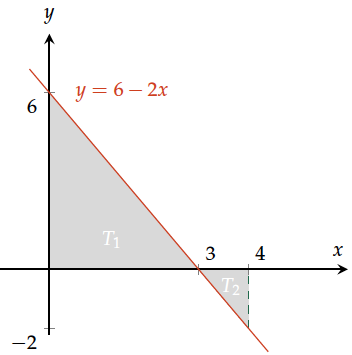
\includegraphics{definArea}
	
	\item Calculate T1, T2 and add them together
	
	$$T_1 = \frac{6 \cdot 3}{2} = 9 \quad T_2 =-\frac{2}{2} = -1 $$
	$$\int_0^4 6-2x \ dx = T_1 + T_2 = 8$$
	
\end{enumerate}
}

\subsubsection{Properties of definite integrals}

\begin{enumerate}
	\item Linearity
	\begin{enumerate}
		\item {$\int_a^b \left( f(x) + g(x)\right) \ dx = \int_a^b f(x) \ dx + \int_a^b g(x) \ dx $}
		\item {$\int_a^b k f(x) \ dx = k \int_a^b f(x) \ dx$}
	\end{enumerate}
	
	\item {$\int_a^b f(x) \ dx = - \int_b^a f(x) \ dx $}
	\item{ $\int_a^a f(x) \ dx = 0$ \label{intprop:b}}
	\item {$\int_a^b f(x) \ dx = \int_a^c f(x) \ dx + \int_c^b f(x) \ dx$ , splitting it into separate limits}
	\begin{figure}[!h]
\centering
\includegraphics[width=0.5\textwidth]{intpropSplit}
\end{figure}

	\item{$\int_a^b k \ dx = k(b-a)$ , integral of a constant = area of rectangle}
	
\begin{figure}[!h]
\centering
\includegraphics[width=0.5\textwidth]{intpropConstant}
\end{figure}

	\item {$\int_a^b \left(f(x) - g(x)\right) dx$, area between two curves}
\begin{figure}[!h]
\centering
\includegraphics[width=0.5\textwidth]{intprop2Curves}
\end{figure}

\end{enumerate}
\newpage
\subsection{Fundamental Theorems of Integral Calculus}

\subsubsection{First FToC}
\par{Let $A(x)$ be a function representing the area under a curve $f(t)$ between a fixed point $a$, and a \ita{variable} point $x$}

$$ A(x) = \int_{a}^{x} f(t) \ dt$$

\begin{theorem} $$A' (x) = f(x)$$ ~\label{ftoc:1} \end{theorem}

\proofs{

\par{For $A(x)$ we have the following difference quotient:}

\mymarginpar{TODO}

}

\subsubsection{Antidifferentiation}

\defn{Antiderivative F(x)}{, for a given $f(x)$ $$ \frac{d}{dx} F(x) = f(x) , \text{  for } x \in I$$}

\begin{theorem}Any antiderivative of $f(x)$ can be written as $F(x) + k$ , for some constant $k$~\label{ftoc:anti}\end{theorem}

\ex{ Let $f(x) = x^4$ , note that any constant when differentiated gives us $0$, hence:

$$ F(x) = \frac{1}{5}x^5 + \text{("any constant") } k$$
}

\subsubsection{Second FToC}

\nota{ $\left[F(x)\right]^{b}_{a} = F(b) - F(a)$}

\begin{theorem}$$\int_{a}^{b} = F(b) - F(a)$$~\label{ftoc:2}\end{theorem}

\proofs{

\par{ By (\ref{ftoc:1}) we know that $A(x)$ is an antiderivative of $f(x)$, and (\ref{ftoc:anti}) tells us that for any other antiderivative $F(x) , \in [a,b]$, then they differ only by a constant, i.e:}

$$F(x) = A(x) + k$$

Therefore, the difference between any two points of $F(x)$ and $A(x)$ is constant, such that:

$$F(a) = A(b) + k \text{ and } F(b) = A(b) + k$$


\par{Therefore:}

\begin{align*}
	\left[F(x)\right] &= F(b) - F(a) \\
		&= (A(b) + c) - (A(a) + c) \\
		&= A(b) - \underbrace{A(a)}_{= 0 , \text{ by } (\ref{intprop:b})}\\
		&= A(b)\\
		&= \boxed{\int_{a}^{b} f(t) \ dt}
\end{align*}
}

\ex{ Find $\int_{0}^{2} (x^3 - x) \ dx$

\begin{enumerate}

	\item{Separating the function by the linearity property}
	
	$$ \int_{0}^{2} (x^3 - x) =  \int_{0}^{2} (x^3) \ dx -  \int_{0}^{2} (x) \ dx$$
	
	\item{Finding the antiderivatives}
	
	$$F(x) = \frac{1}{4}x^4 \text{ and } G(x)=\frac{1}{2}x^2$$
	
	\item{Evaluating the integrals, by FToC2 (\ref{ftoc:2})}
	
	$$\left[F(x)\right]^{2}_{0} = \frac{1}{4}2^4 - \frac{1}{4}0^4 = 4 \text{ and } \left[G(x)\right]^{2}_{0} = \frac{1}{2}2^2 - \frac{1}{2}0^2 = 2$$
	
	$$\int_{0}^{2} (x^3 - x) \ dx = 4 - 2 = 2$$
\end{enumerate}

}

\subsection{Differentiation and Integration as Inverse Processes}

\defn{Definite Integral}{$ \int f(x) dx = F(x) + C$}
\newpage
\ex{Verify the Standard Integral (SI) $$\int \frac{1}{\sqrt{a^{2}-x^{2}}} d x=\sin ^{-1}\left(\frac{x}{a}\right)+c, \quad a>0$$ \\

\par{We have that }$$ \frac{d}{dx} \left[\sin ^{-1}\left(\frac{x}{a}\right)\right] = \frac{1}{\sqrt{1-(\tfrac{x}{a})^2}} \cdot \frac{d}{dx} \left(\frac{x}{a}\right) = \frac{1}{\sqrt{a^{2}-x^{2}}} $$

\par{Hence, $\int \frac{1}{\sqrt{a^{2}-x^{2}}} d x=\sin ^{-1}\left(\frac{x}{a}\right)+c, \quad a>0$}
}


\prop{Linearity }{Integration is linear}

\proofs{$$\begin{aligned} \frac{d}{d x}\left[\int f(x) d x+\int g(x) d x\right] &=\frac{d}{d x}\left(\int f(x) d x\right)+\frac{d}{d x}\left(\int g(x) d x\right) \\ &=f(x)+g(x) \end{aligned} $$\\ So, given that the sum of the integrals is an anti-derivative of $f(x) + g(x)$. We have that:

$$\int(f(x)+g(x)) d x=\int f(x) d x+\int g(x) d x$$
}

\newpage

\section{Techniques of Integration}

\subsection{Substitution}

\par{Let $F(x)$ be the antiderivative with respect to $x$ of $f(x)$, i.e $F'(x) = f(x)$. Then, if $u = g(x)$ we can rewrite the new integral in terms of $u$.}

\begin{theorem}$$\int f(g(x)) g^{\prime}(x) d x=\int f(u) \frac{d u}{d x} d x=\int f(u) d u=F(u)=F(g(x))$$\end{theorem}

\proofs{Chain Rule, $$\frac{d}{d x} F(g(x))=F^{\prime}(g(x)) \frac{d}{d x} g(x)=f(g(x)) g^{\prime}(x)$$
$$ \int f(g(x)) g^{\prime}(x) d x=F(g(x))+c$$}

\rem{It's a technique closely related to the chain rule}

\rem{If there are still $x$ terms left after the substitution, it is often necessary to rewrite $x$ in terms of $u$}

\rem{For definite integrals, one must also substitute the limits of integration for values of $u$, by evaluating $g(x)$, where $x$ is the original limit}

\subsection{By Parts}

\begin{theorem}$$ \int u \frac{dv}{dx}\ dx = uv - \int v\frac{du}{dx}\ dx $$
$$ \equiv $$
$$ \int u \ dv = uv - \int v \ du $$\end{theorem}

\rem{Closely related to the product rule}

\rem{When deciding on which function to make equal to $u$ , follow the rule of thumb L.I.A.T.E}

\subsection{Trigonometric}

\subsubsection{Squares} 

\par{Remember the following identities:}

$$\tan^{2}(x) = \sec^{2}(x) - 1 \quad \cos^{2}(x)+\sin^{2}(x) = 1 \quad \cos^{2}(x) = \frac{\cos(2x) + 1}{2} \quad \sin^{2}(x) = \frac{1 - \cos(2x)}{2}$$

\par{Then:}

\begin{itemize}
\item[] $\int \tan ^{2} x d x=\int\left(\sec ^{2} x-1\right) d x=\tan x-x+c$
\item[] $\int \cos ^{2} x d x=\int \frac{1}{2}+\frac{1}{2} \cos 2 x d x=\frac{1}{2} x+\frac{1}{2} \cdot \frac{1}{2} \sin 2 x+c=\frac{1}{2} x+\frac{1}{4} \sin 2 x+c$
\item[] $\int \sin ^{2} x d x=\int \frac{1}{2}-\frac{1}{2} \cos 2 x d x=\frac{1}{2} x-\frac{1}{4} \sin 2 x+c$
\end{itemize}

\subsubsection{Irreducible Quadratic}

\par{For integrals of the type $\frac{1}{\text{irreducible quadratic}}$. First one completes the square, and then applies the standard integral $$ \int \frac{1}{x^{2}+a^{2}} d x=\frac{1}{a} \tan ^{-1}\left(\frac{x}{a}\right)+c $$}

\ex{$$\begin{aligned} \int \frac{1}{x^{2}+x+1} d x &==\int \frac{1}{\underbrace{\left(x+\frac{1}{2}\right)^{2}}_x+\underbrace{\frac{3}{4}}_{a^2}} d x \\ &=\frac{2}{\sqrt{3}} \tan ^{-1}\left(\frac{x+\frac{1}{2}}{\frac{\sqrt{3}}{2}}\right)+c \\ &=\frac{2}{\sqrt{3}} \tan ^{-1}\left(\frac{2 x+1}{\sqrt{3}}\right)+c \end{aligned}$$}

\subsubsection{Of the form: $\int \sin ^{m} x \cos ^{n} x d x, m, n \in \mathbb{Z}^{+}$}

\begin{itemize}
	\item[] $m$ even, $n$ odd : Let $u = \sin(x)$
	\item[] $m$ odd, $n$ even: Let $u = \cos(x)$
	\item[] both odd : any will do, but sometimes one might be easier
	\item[] both even (see example) : In general, for higher powers, the repeated application of trig identities, can be repeatedly applied to obtain the required integral
	\end{itemize}
	
\ex{ Considering the identites:
$$ \sin 2 x=2 \cos x \sin x \quad \quad \text{ and } \quad \quad \sin ^{2} x=\frac{1-\cos 2 x}{2}$$
Then,  $$\begin{aligned} \int \sin ^{2} x \cos ^{2} x d x=\int\left(\frac{1}{2} \sin 2 x\right)^{2} d x &=\frac{1}{4} \int \sin ^{2}(2 x) d x \\ &=\frac{1}{4} \times \frac{1}{2} \int 1-\cos 4 x d x \\ &=\int \frac{1}{8}-\frac{1}{8} \cos 4 x d x \\ &=\frac{1}{8} x-\frac{1}{32} \sin 4 x+c \end{aligned}$$}

\subsubsection{Trig Substitutions} 

\par{Let $a > 0$, and a constant}

\begin{enumerate}
\item For $(a^{2} - x^{2})^{n}$ , apply the substitution $\boxed{x = a\sin\theta}$. So that,

$$a^{2} - (a\sin\theta)^{2} = a^{2}\cos^{2}\theta \quad \text{ and } \quad dx = a\cos\theta d\theta$$

\item For $(a^{2} + x^{2})^{n}$ , apply the substitution $\boxed{ x = a\tan\theta}$. So that,

$$a^{2} + (a\tan\theta)^{2} = a\sec^{2}\theta \quad \text{ and } \quad dx = a\sec^{2}\theta $$

\end{enumerate}
\subsection{Logarithmic}

\begin{theorem} $$ \int \frac{f^{\prime}(x)}{f(x)} d x=\log |f(x)|+c $$ \end{theorem}

\proofs{
\par{Observe, by using the chain rule that for $\frac{d}{d x}(\log |f(x)|), \text { if } f(x)>0$: }
$$\frac{d}{d x}(\log f(x))=\frac{f^{\prime}(x)}{f(x)}$$

\par{Hence, for $f(x) < 0$:}
$$\frac{d}{d x}(\log (-f(x)))=\frac{-f^{\prime}(x)}{-f(x)}=\frac{f^{\prime}(x)}{f(x)}$$

\par{Therefore, $\log|f(x)|$ is an antiderivative of $\frac{f'(x)}{f(x}$}
}

\subsection{Rational Functions} 

\mymarginpar{Recall: Proper $\iff \frac{p(x)}{q(x)}$ , deg $p < \text { deg } q$}

\begin{enumerate}

\item Write as the sum of a proper rational and polynomial
\item Expand newly found rational into partial fractions \mymarginpar{For non-expandable (e.g. irreducible quadratics) it might be needed to complete the square, before applying a trig substitution}
\item Integrate each term as \ita{per usual}

\end{enumerate}

\ex{$ \int \frac{x^{3}-4}{x^{2}-x-2} d x$

\mymarginpar{See 3.18/19 lec notes for +examples}

\begin{enumerate}
\item 
$$\polylongdiv{x^{3}-4}{x^{2}-x-2}$$

\item

$$\frac{3x-2}{x^{2}-x-2} = \frac{4}{3(x-2)} + \frac{5}{3(x+1)}$$

\item*

$$\int \frac{x^{3}-4}{x^{2}-x-2} \ d x = \int \left[ (x+1) + \frac{4}{3(x-2)} + \frac{5}{3(x+1)} \right] \ d x$$\mymarginpar{*Then apply S.I}
\end{enumerate}

}




 

\section{Symmetry and Definite Integrals} \mymarginpar{ $t = -x$}

\defn{Even}{ $f(x)$ is even if $f(x) = f(-x)$ for all $x$}

$$\begin{aligned} \int_{-a}^{a} f(x) d x &=\int_{-a}^{0} f(x) d x+\int_{0}^{a} f(x) d x \\ &=-\int_{a}^{a} f(t) d t+\int_{0}^{a} f(x) d x \\ &=2 \int_{0}^{a} f(x) d x \end{aligned}$$

\defn{Odd}{ $f(x)$ is odd if $-f(x) = f(-x)$ for all $x$}

$$\begin{aligned} \int_{-a}^{a} f(x) d x &=\int_{-a}^{0} f(x) d x+\int_{0}^{a} f(x) d x \\ &=-\int_{a}^{0}-f(t) d t+\int_{0}^{a} f(x) d x \\ &=0 \end{aligned}$$

\ex{ Determine the parity of $f(x)=5 x^{7}+7 x^{3}+9 x^{5}$. We have that:

\begin{align*}
f(-x) &=  5(-x)^{7}+7 (-x)^{3}+9 (-x)^{5} \\
&= -5x^7 -7x^3 -x^5 \\
&= -(5 x^{7}+7 x^{3}+9 x^{5})\\
&= -f(x)
\end{align*}

Hence, odd.
}

\section{Ordinary Differential Equations}

\defn{ODE}{Equation which relates a function $y(x)$ , $x$ and at least one $n^{th}$ derivative of $y$ with respect to $x$, i.e. $\frac{d^{n}y}{dx^{n}}$}

\rem{The order of an ODE is given by the degree of its highest derivative}

\defn{Linear ODE}{An ODE where there are no (1) products of $y$ and its derivatives (2) no functions of $y$ and its derivatives}

\ex{ 
\begin{itemize}
\item[]
\item $y + \frac{dy}{dx} = xy$ \quad \quad LODE
\item $y^2 + \frac{dy}{dx} = xy$ \quad \quad Not Linear ($y \times y$)
\item $\cos(y) + \frac{dy}{dx} = xy$ \quad \quad Not Linear ($\cos(y)$)
\end{itemize}
}

\subsection{Separable}

\defn{Separable ODE}{An ODE is said to be separable if it can be written in the form $\frac{dy}{dx} = f(x)g(y)$}

\par{To solve $1^{\text{st}}$ order ODEs, all it needs to be done is to \ita{"split"} the \ita{"y's"} and \ita{"x's"} into each side of the equation, and integrate for the respective variable}

\ex{ 
\begin{align*}
\frac{dy}{dx} &= (6x^2 +1)y  \\
\int \frac{1}{y} \ dy &= \int 6x^2 + 1 \ dx \\
log|y| &= 2x^3 + x + C \\
y &= e^{2x^3 + x + C} = C^{*}e^{2x^3 + x}
\end{align*}
}\mymarginpar{* $e^C$ is just a constant}

\subsection{Integration Factor}

\defn{Integrating Factor ( $\mu(x)$ )}{Factor which when multiplied by the LHS of a general linear ODE, transforms it into the total derivative $\frac{d}{dx}\left(\mu(x)y(x)\right)$}

\defn{Standard Form  }{$\boxed{\frac{dy}{dx} + p(x)y(x) = \lambda(x)}$ , where $\lambda(x)p(x)$ are functions of $x$ only}

\rem{In general $\mu(x) = e^{\int p(x) dx}$ , see 4.7 lecture notes for full derivation}

\begin{itemize}
\item[]\textbf{Method:}
\begin{enumerate}
	\item Make sure that the ODE is in standard form 
	\item Find the Integrating Factor $\mu(x)$
	\item Multiply standard ODE by $\mu(x)$ in order to transform the LHS into the total derivative $\frac{d}{dx}\left(\mu(x)y(x)\right)$
	\item Integrate both sides
	\item Solve for $y(x)$
\end{enumerate}
\end{itemize}

\rem{Note that when integrating the LHS, the integration and differential operators will simply cancel out}

$$ \mu(x) = exp\left(\int{\frac{x+2}{x}}\right) = e^xx^2 \quad \quad (2)$$
\ex{ 
\begin{alignat*}{2}
&\frac{dy}{dx} +\left( \frac{x +2}{x}\right)y = e^{-x} \quad \quad &(1)\\
&\frac{d}{dx}\left[(e^xx^2)(y)\right] = e^{-x}(e^xx^2) \quad \quad &(3)\\
&e^xx^2(y) = \int{x^2} \quad \quad &(4) \\
&y = {e}^{-x}\left( \frac{1}{3}x + \frac{C}{x^2} \right) \quad \quad &(4) , (5)
\end{alignat*}{2}
}

\subsection{Second Order ODEs}

$$ \text{General Form: } p(x)y'' + q(x)y' + r(x)y = f(x)$$

\par{At this level, priority is given to the simpler form of the above (Constant 2ODE), where the functions with respect to $x$ have no variables, i.e. $p(x),q(x),r(x)$  are constants}

\defn{Homogeneous}{An ODE is said to be homogeneous if it is composed only of $y$ and its derivatives, i.e. if $f(x) = 0$}

\defn{Non-Homogenous}{An ODE with functions other than $y$, i.e. $f(x) \neq 0$}

\ex{ H : $y'' + 5y' + 6y = 0$ \quad \quad NH: y'' + 5y' + 6y = 3x}

\begin{theorem}{\textbf{Superposition: }}{If $y_1(x)$ and $y_2(x)$ are both solutions of a \ita{linear} homogenous ODE, so it is any linear combination of them $$y(x) = c_1y_1(x) + c_2y_2(x)$$}\end{theorem}

\subsubsection{Characteristic/Auxiliary Equation}

\par{To understand the concept of a characteristic equation, its best if we start with an example. Note the following second order linear homogenous ODE:}

$$y'' + 5y' + 6y = 0$$

\par{We know that there is some function $g(x)$ which solves the above. In this case the solution seems to be simple, maybe a function whose derivatives vary only in its coefficients. A common example given in the literature is to take $g(x) = e^{rx}$. Let's then, by inspection,  see if its simplest form $e^x$ could be a solution:}

$$ (e^x)'' = e^x \quad \quad (e^x)' = e^x $$

\par{Hence, for $g(x) = e^x$, we have that,}

$$e^x + 5e^x + 6e^x = 12e^x \neq 0 \ \forall \  x , \text{ hence not a solution}$$

\par{So, $r=1$ does not satisfy the equation. We can then ask ourselves if there's any value of $r$ which could. In order to find it, all we need to do is to essentially solve for $r$. Repeating the process above:}

$$(e^{rx})'' = (re^{rx})' = r^2e^rx \quad \quad (e^{rx})' = re^{rx}$$

\par{Hence, for $g(x) = e^{rx}$, we have that}
$$r^2e^rx + 5(re^{rx}) + 6e^{rx} = 0 \iff e^{rx} \boxed{(r^2 + 5r + 6)} = 0$$

\par{Note that $e^{rx}$ is never $0$ , hence we find our $r$(s) by solving the quadratic boxed above. It is that quadratic which we call the \textbf{\ita{characteristic equation}} of a 2ODE , and the polynomial on the left its \textbf{\ita{characteristic polynomial}}.\\
So, finding the roots to specify $r$, and by the superposition principle defined above, we can define the GS for our example}

$$y(x) = C_1e^{-2x} + C_2e^{-3x}$$

\par{\textbf{In General:} if $r$ satisfies the characteristic equation $pr^2 + qr + n$ , then $e^{rx}$ is a solution of the 2ODE\mymarginpar{PS ($C_1, C_{2}$) are found by solving for 2 initial conditions instead of one}}

\par{The GS can take different forms, depending on the roots of the CE}

\begin{enumerate}
	\item Distinct : $C_1e^{r_1x} + C_2e^{r_2x} $
	\item Repeated : $C_1e^{r_1x} + C_2xe^{r_2x}$
	\item Complex $(\alpha \pm i\beta)$ : $e^{\alpha x}\left(A\cos(\beta)x + B\sin(\beta)x\right)$
\end{enumerate}

\subsubsection{Particular Integrals}

\par{To construct particular solutions for \ita{non-homogenous} equations one starts by using a general, functionally equal $g(x)$ to $f(x)$, i.e. for a trig function, use general trig, poly to poly etc.}

\ex{ Find GS for $y'' + 3y' + 2y = 6e^{2x}$

\begin{enumerate}

\item LHS is Homogeneous, hence we know:

$$\text{CE: } r^{2} + 3r + 2 = 0 \iff r = -2 , -1$$
$$y(x) = Ae^{-2x} + Be^{-x}$$

\item RHS is NH and of exponential type, hence

$$y = Ae^{Bx} \quad y' = ABe^{Bx} \quad y'' = AB^{2}e^{Bx}$$

\item Substituting in original ODE

$$(AB^{2}e^{Bx}) + 3ABe^{Bx} + 2Ae^{Bx} = 6e^{2x}$$

\item Equating LHS\&RHS Coefficients

$$B = 2 \quad \text{ and } \quad 4Ae^{2x} + 6Ae^{2x} + 2Ae^{2x} = 6e^{2x} \iff A = \frac{1}{2}$$
Hence, we have that
$$ \frac{1}{2}e^{2x} $$

\item Finally, by the superposition principle, given that both are solutions, their linear combination must also be

$$y(x) =  Ae^{-2x} + Be^{-x} + \frac{1}{2}e^{2x} $$

\end{enumerate}
}

\newpage
\nocite{*}
\printbibliography

\end{document}

